
\documentclass[a4paper]{article}

\usepackage{fullpage}
\usepackage[frenchb]{babel}
\usepackage[T1]{fontenc}
\usepackage{times}
\usepackage[utf8]{inputenc}
\usepackage{verbatim}
\usepackage{amsmath}
\usepackage{graphicx}
\usepackage{caption} 
\usepackage{amsthm}
\usepackage{float}
\usepackage{amssymb}

\theoremstyle{definition}
\newtheorem{que}{Question}


\title{Compte-rendu de TP de méthode numérique de base}
\author{Maxime Gourgoulhon \and Pierre Bouvier}

\begin{document}
	\maketitle
	\begin{que}
		D'après (10), pour $k \in \mathbb{N}$ et $i \in 1..n$:
		\begin{align*}
			(10) \Leftrightarrow \frac{u_i^{(k+1)} - u_i^{(k)}}{\delta_t} = \frac{\theta}{\delta_x^2} [C_{i+1/2}u_{i+1}^{(k+1)} - (C_{i+1/2} + C_{i-1/2})u_{i}^{(k+1)} + C_{i-1/2}u_{i-1}^{(k+1)}]
\\ + \frac{1-\theta}{\delta_x^2} [C_{i+1/2}u_{i+1}^{(k)} - (C_{i+1/2} + C_{i-1/2})u_{i}^{(k)} + C_{i-1/2}u_{i-1}^{(k)}] \\
\Leftrightarrow u_i^{(k+1)} + \theta\frac{\delta_t}{\delta_x^2} [-C_{i+1/2}u_{i+1}^{(k+1)} + (C_{i+1/2} + C_{i-1/2})u_{i}^{(k+1)} - C_{i-1/2}u_{i-1}^{(k+1)}] \\ =  u_i^{(k)}
+(\theta-1)\frac{\delta_t}{\delta_x^2}[-C_{i+1/2}u_{i+1}^{(k)} + (C_{i+1/2} + C_{i-1/2})u_{i}^{(k)} - C_{i-1/2}u_{i-1}^{(k)}]
		\end{align*}

		Posons la matrice A suivante (attention à l'alignement des lignes obliques):
		\begin{align*}
			A=
			\begin{pmatrix}
				C_{1-1/2} + C_{1+1/2} & - C_{1+1/2}  & 0 & \cdots & \cdots & 0 \\
				 - C_{2-1/2} & C_{2-1/2} + C_{2+1/2} & - C_{2+1/2}  & \ddots & ~ & \vdots\\
				0 & - C_{3-1/2} & C_{3-1/2} + C_{3+1/2} & - C_{3+1/2}  & \ddots & \vdots\\
				\vdots & \ddots & \ddots & \ddots & \ddots & 0\\
				\vdots & ~ & \ddots & \ddots & \ddots & - C_{(n-1)+1/2}\\
				0 & \cdots & \cdots & 0 & - C_{n-1/2} & C_{n-1/2} + C_{n+1/2} \\
			\end{pmatrix}
		\end{align*}

		Pour $i \in 2..(n-1)$, d'après le système précédent, le schéma (11) de l'énoncé est vérifié.
		En effet, à chaque ligne i du schéma (10) correspond à notre système, pour le même i fixé.\\

		Pour $i = n$, on a $u_{n+1}^{(t)} = 0$. Ainsi on peut simplifier le système de notre rendu en éliminant les $u_{n+1}^{(t)}$.
		Au final, la dernière ligne n du schéma matriciel de l'énoncé correspond à notre équation. \\

		Pour $i = 0$, on a $u_0^{(t)} \ne 0$. Autrement dit, il faut rajouter un terme supplémentaire.
		L'énoncé l'a fait pour nous, en posant $B_i^{(k)}$
		En effet, contrairement au cas $i=n$, l'absence de $u_0^{(t)}$ dans $U^{(k)}$ changerait le système de notre rendu pour $i=0$. \\

		On en déduit que le schéma s'écrit de façon matricielle, avec notre matrice A posée et (11) de l'énoncé. \\

		A est tridiagonale. \\

		A est symétrique (en effet $\forall k, C_{k-1/2} = C_{x_k - \delta / 2} = C_{\delta (k - 1/2) - l} = C_{(k-1)+1/2}$). \\
		Cela démontre aussi que la notation adoptée par l'énoncé pour les $C$ est sans ambiguité. \\

		Conclusion: La matrice A définie précédemment est alors symétrique, tridiagonale et satisfait l'équivalence entre (10) et (11) de l'énoncé. \\
	\end{que}
	\begin{que}
		Montrons que A est définie-positive.
		Soit $ x = {}^t \begin{pmatrix} x_1 & x_2 & \cdots & x_{n-1} & x_n \end{pmatrix}$ non-nulle. \\
		Montrons que ${}^txAx > 0$
		\begin{align*}
			Ax=
			\begin{pmatrix}
				(C_{1-1/2} + C_{1+1/2}) x_1 - C_{1+1/2} x_2 \\
				 - C_{2-1/2} x_1 + (C_{2-1/2} + C_{2+1/2}) x_2 - C_{2+1/2} x_3 \\
				\vdots \\
				- C_{i-1/2} x_{i-1} + (C_{i-1/2} + C_{i+1/2}) x_i - C_{i+1/2} x_{i+1} \\
				\vdots \\
				- C_{n-1/2} x_{n-1} + (C_{n-1/2} + C_{n+1/2}) x_n \\
			\end{pmatrix}
		\end{align*}
		Par commodité, posons $ x_0 = x_{n+1} = 0$
		\begin{align*}
			{}^txAx=\sum_{i=1}^n (- C_{i-1/2} x_{i-1} + (C_{i-1/2} + C_{i+1/2}) x_i - C_{i+1/2} x_{i+1}) x_i \\
			= C_{1/2} x_1^2 + C_{n+1/2} x_n^2 + \sum_{i=1}^{n-1} C_{i+1/2} (x_i - x_{i+1})^2 \\
		\end{align*}
		On remarque directement que ${}^txAx \ge 0$.
		Il reste ainsi à montrer que ${}^txAx \ne 0$. \\
		Par l'absurde, si ${}^txAx=0$, alors:
		$x_1 = 0$, $x_n = 0$ et $\forall i \in [1..n-1], x_i = x_{i+1}$ \\
		Autrement dit $x = 0$. D'où la contradiction. \\
		Conclusion: A est définie-positive.
	\end{que}
	\setcounter{que}{5}
	\begin{que}
		Reprenons le schéma (10) de l'énoncé et les résultats de la question 1. \\

		Comme le problème est stationnaire, on a: $\forall k \in [0, T],  U^{(k)}=U^{(k+1)}$ \\
		Nous noterons ce vecteur $U$. \\

		Comme le problème est stationnaire et par la même argumentation, $B^{(k)}$ ne dépend pas de k. Nous noterons ce vecteur $B$. \\

		D'après la question 1, pour $k \in \mathbb{N}$ et $i \in 1..n$: \\
		$(I + \theta \mu A)U = (I + (\theta - 1) \mu A)U^{(k)} + \mu B^{(k)}$ \\
		$\Leftrightarrow 0 = (( - 1) \mu A)U + \mu B$ \\
		$\Leftrightarrow AU = B$ car $\mu$ non-nul \\
		Comme $A$ est définie-positive, alors $A$ est inversible, donc $A$ est une bijection de $\mathbb{R}^n$ sur $\mathbb{R}^n$. \\
		Ainsi $U$ admet une unique solution dans l'équation $AU=B$.\\
		D'où le résultat. \\
	\end{que}
	\begin{que}
		On réécrit le système avec $C(x)=exp(-x/l)$ et $u_0 = 1$: \\
		$(13) \Leftrightarrow \frac{\delta^2 u}{\delta^2 x} l = \frac{\delta u }{\delta x}$ car $\forall x, C(x) \ne 0$ et $C'(x) \ne 0$\\
		Les solutions sont: $ \frac{\delta u }{\delta x} = k exp(x/l)$ où ($k \in \mathbb{R}$). \\
		Ainsi $u(x) = a + b exp(x/l)$ avec $a, b \in \mathbb{R}$. \\
		On fixe les constantes avec les conditions initiales: $b=\frac{1}{e^{-1}-e}$ et $a=-eb$. \\
		La solution est donc $u(x)=\frac{e^{x/l}-e}{e^{-1}-e}$ pour $x \in [-l, l]$.\\
		\begin{center}
		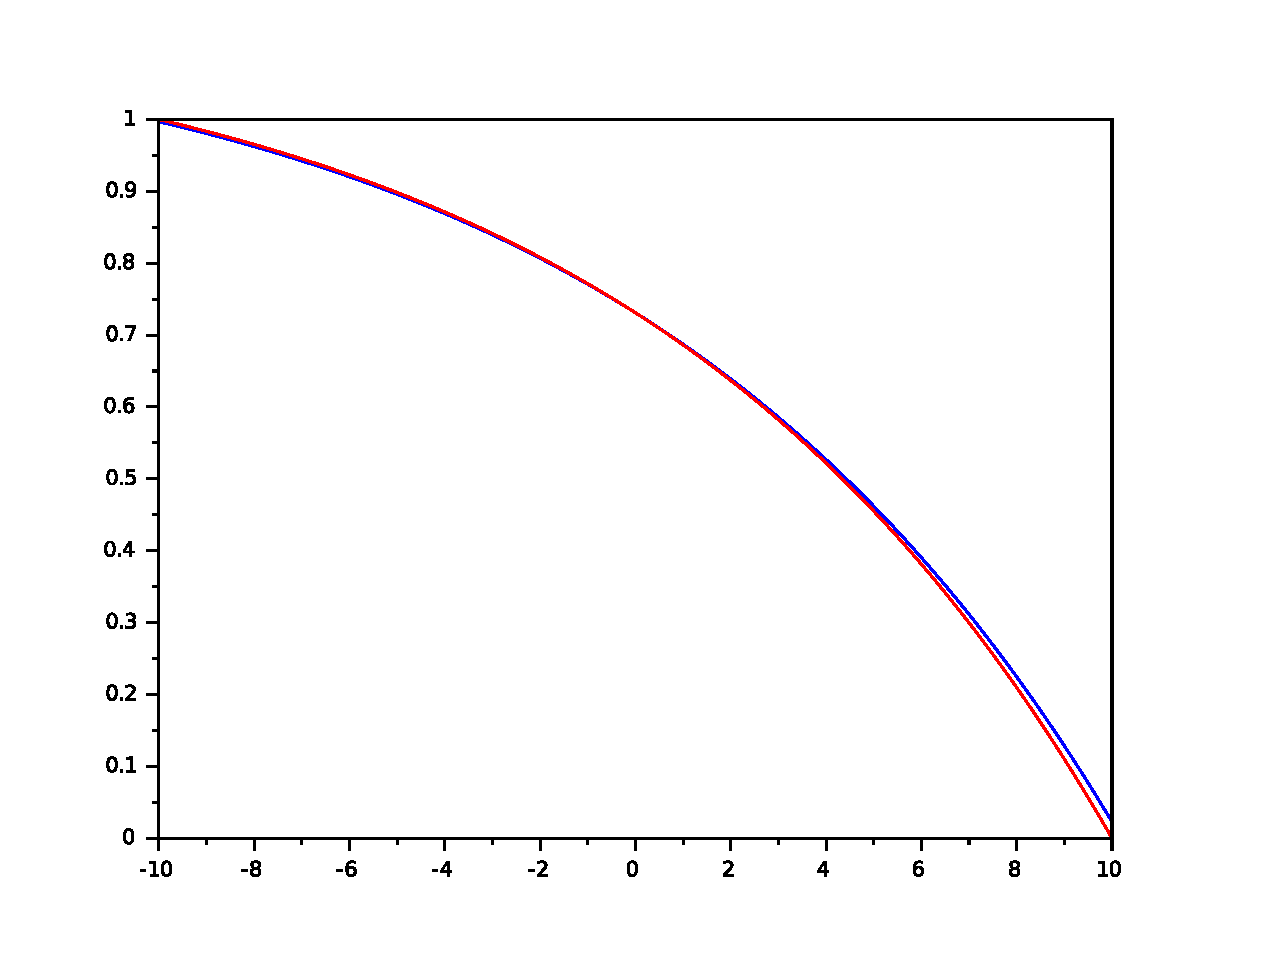
\includegraphics[width=15cm]{graphes/q7.pdf}
		\captionof{figure}{Comparaison entre la solution explicite (en rouge) et la solution numérique (en bleu)}
		\label{fig1}
		\end{center}
	\end{que}
	\begin{que}
		A étant définie-positive, elle est inversible, et comme $\mu \theta \leq 0$ alors M est inversible. \\
		Montrons que $M^{-1}N$ et $A$ ont les mêmes vecteurs propres: \\
		Soit $x \neq 0$ vecteur propre associée à la valeur propre $\lambda$.
		On a alors: \\
		$M^{-1}Nx=\lambda x \Leftrightarrow Nx=\lambda Mx$
		$\Leftrightarrow x +(\theta - 1) \mu A x = \lambda x + \theta \mu \lambda Ax$
		$\Leftrightarrow  Ax = \frac{(1 - \lambda)}{\mu(1+\theta(\lambda - 1))} x$ \\
		On a une équivalence, ainsi $M^{-1}N$ et $A$ ont les mêmes vecteurs propres.\\
		En revanche pour un vecteur propre $x$ fixé, on a des valeurs propres associées différentes: $\lambda \in Sp(M^{-1}N) \Leftrightarrow \frac{(1 - \lambda)}{\mu(1+\theta(\lambda - 1))} \in Sp(A)$ \\

		Posons $\theta = 1/2$ et "inversons" l'équivalence: \\
		$\frac{1 - \mu \lambda / 2}{1 + \mu \lambda / 2} \in Sp(M^{-1}N) \Leftrightarrow \lambda \in Sp(A)$ \\

		Montrons que $\forall \lambda \in Sp(A), \frac{1 - \mu \lambda / 2}{1 + \mu \lambda / 2} \in ]-1, 1[$ \\
		Puisque: $\mu \ge 0$ et $\lambda > 0$ (Déjà vu) \\
		On a: $ -1 -\mu \lambda/2 < -1 + \mu \lambda / 2 < 1 +\mu \lambda / 2$ \\
		D'où le résultat ($\forall \lambda \in Sp(M^{-1}N), \lambda < 1$) \\

		Ainsi: $\rho(M^{-1}N) = max(Sp(M^{-1}N)) < 1$ \\
		Conlusion: $\rho(M^{-1}N) < 1$
	\end{que}
	\begin{que}
		Le rayon spectral de $M^{-1}N U^{(k)}$ étant strictement inférieur à 1, la méthode (14) converge. \\

		Comme l'addition et le produit de matrices sont des applications continues: \\
		$N\lim\limits_{k \to +\infty} U^{(k)} + \mu B = (\lim\limits_{k \to +\infty} NU^{(k)}) + \mu B = \lim\limits_{k \to +\infty} (NU^{(k)} + \mu B) = \lim\limits_{k \to +\infty} MU^{(k+1)} = M\lim\limits_{k \to +\infty} U^{(k)}$ \\
		On peut alors écrire (en prenant les deux extremités): $(M-N) \lim\limits_{k \to +\infty} U^{(k)}=\mu B$ \\

		On a aussi: $(M-N)^{-1} = A^{-1} / \mu$ \\
		D'où: $\lim\limits_{k \to +\infty} U^{(k)} = BA^{-1}$ \\
		Conclusion: $U^{(k)}$ converge en $+\infty$ vers la solution stationnaire du problème précédent.
	\end{que}
		\begin{center}
		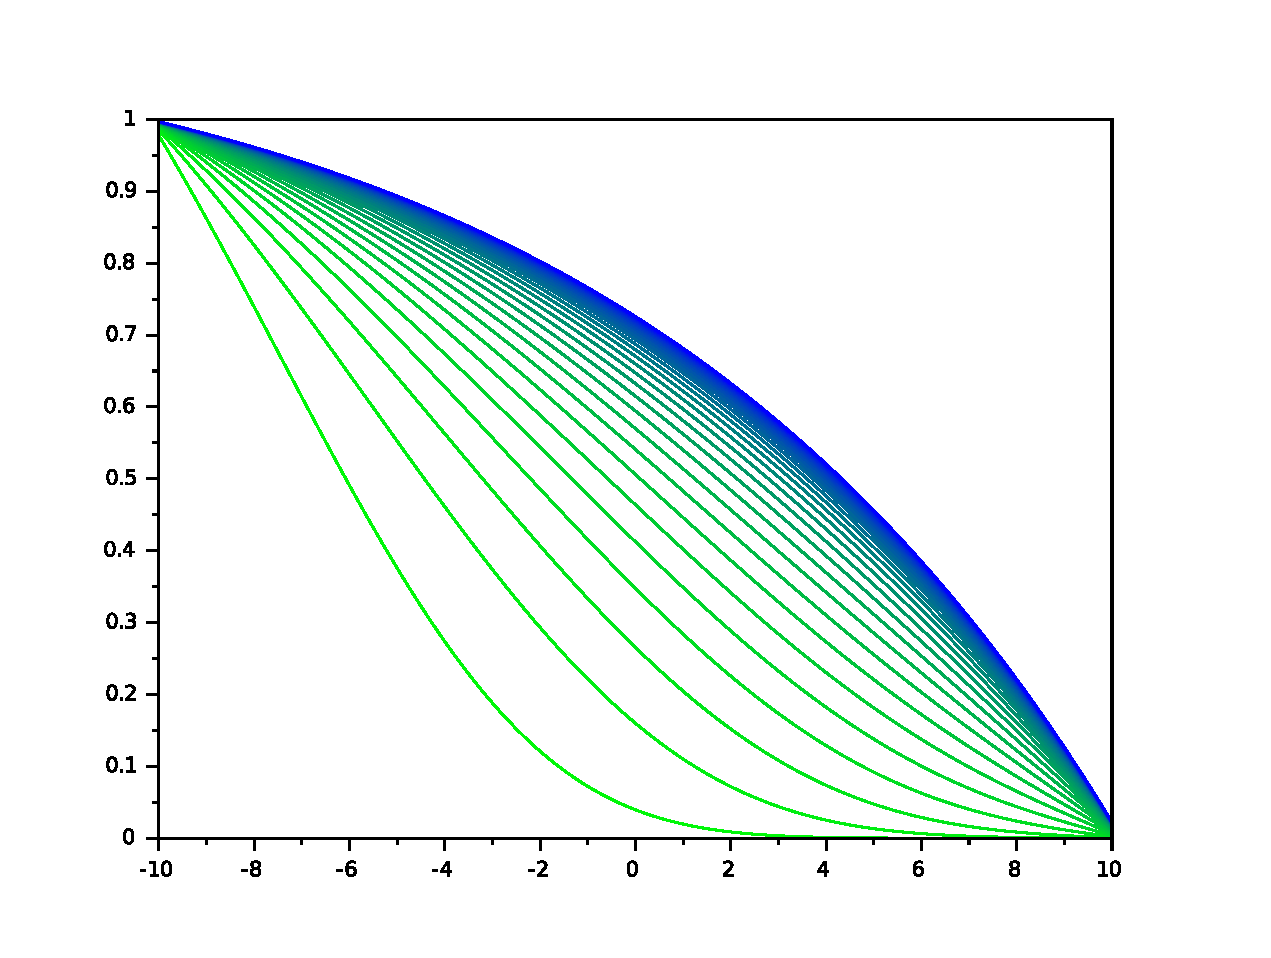
\includegraphics[width=15cm]{graphes/q10.pdf}
		\captionof{figure}{Solution numérique en fonction de $x$ à différents temps $t_k$ fixés}
		\label{fig1}
		\end{center}
	\setcounter{que}{11}
		\begin{center}
		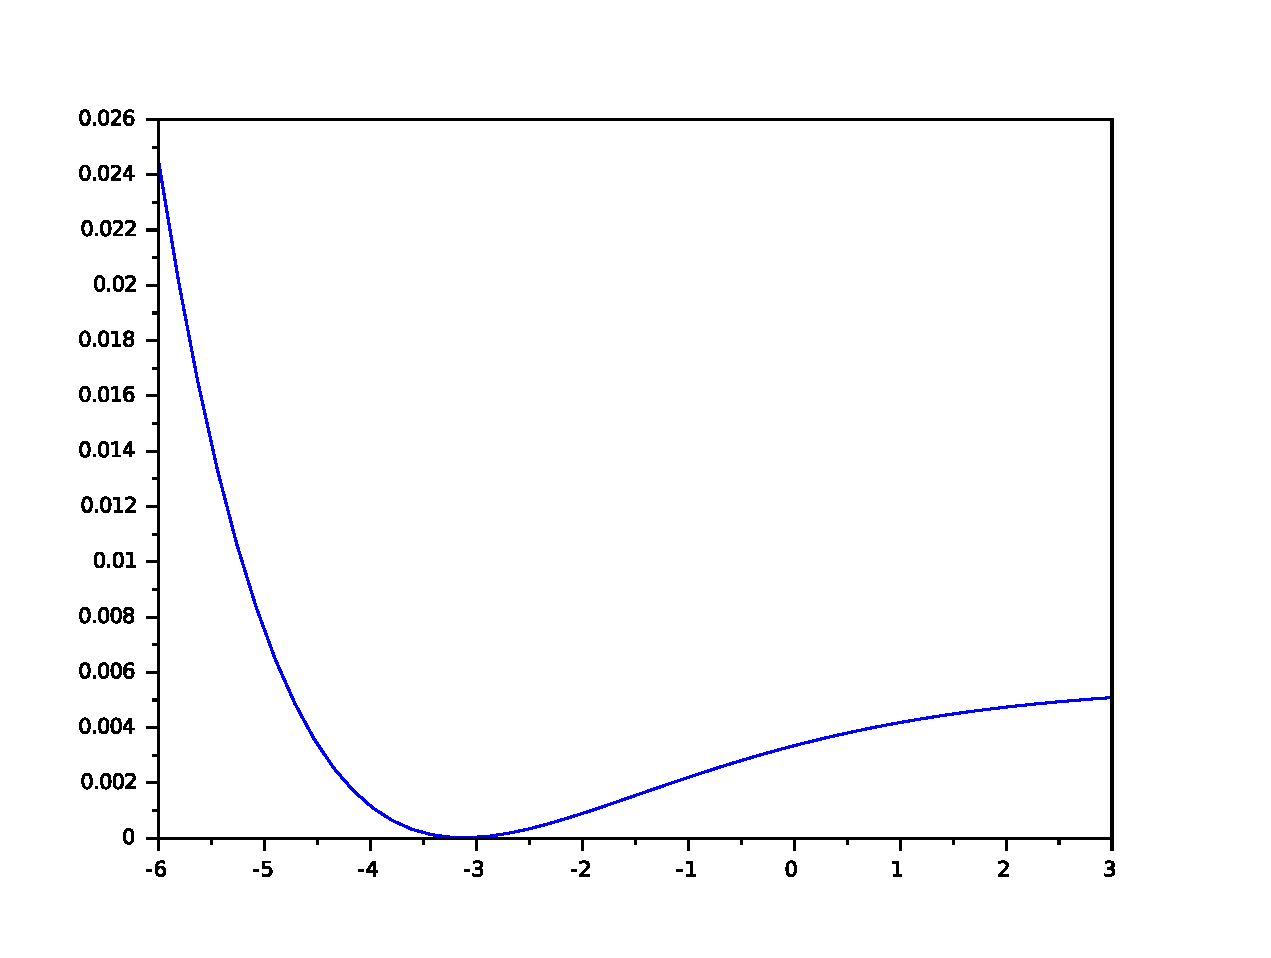
\includegraphics[width=15cm]{graphes/q12.pdf}
		\captionof{figure}{fonction de coût $J$}
		\label{fig1}
		\end{center}
	
	\setcounter{que}{12}
	\begin{que}
		Avec ces trois points, nous avons quatre cas. Pour les résoudre, nous utilisons le fait que le seul minimum de la fonction est $x_d$, que la fonction est strictement décroissante pour $x \leq x_d$, puis strictement croissante pour $x \geq x_d$: \\
		\begin{enumerate}
			\item $J(x1) \leq J(x2) \leq J(x3)$: Le minimum n'étant pas dans $[x_3, b]$, on peut chercher dans $[a, x_2]$
			\item $J(x1) \geq J(x2) \geq J(x3)$:  Le minimum n'étant pas dans $[a, x_1]$, on peut chercher dans $[x_2, b]$
			\item $J(x1) \geq J(x2)$ et $J(x2) \leq J(x3)$: Le minimum étant ni dans $[x_3, b]$, ni dans $[a, x_1]$, on peut chercher dans $[x_1, x_3]$
			\item $J(x1) \leq J(x2)$ et $J(x2) \geq J(x3)$: Ce cas est impossible
		\end{enumerate}
		Et ensuite nous réitérons.
	\end{que}
\end{document}
